\subsection{AI \& Networked Robotics in \proje}

\begin{figure}[!t]
  \centering 
  \subfigure[]{\label{fig:vehicles}\includegraphics[scale=0.075]{fig/vehicles.jpg}}
  \hspace{+0.5cm} 
  % \subfigure[]{\label{fig:agent}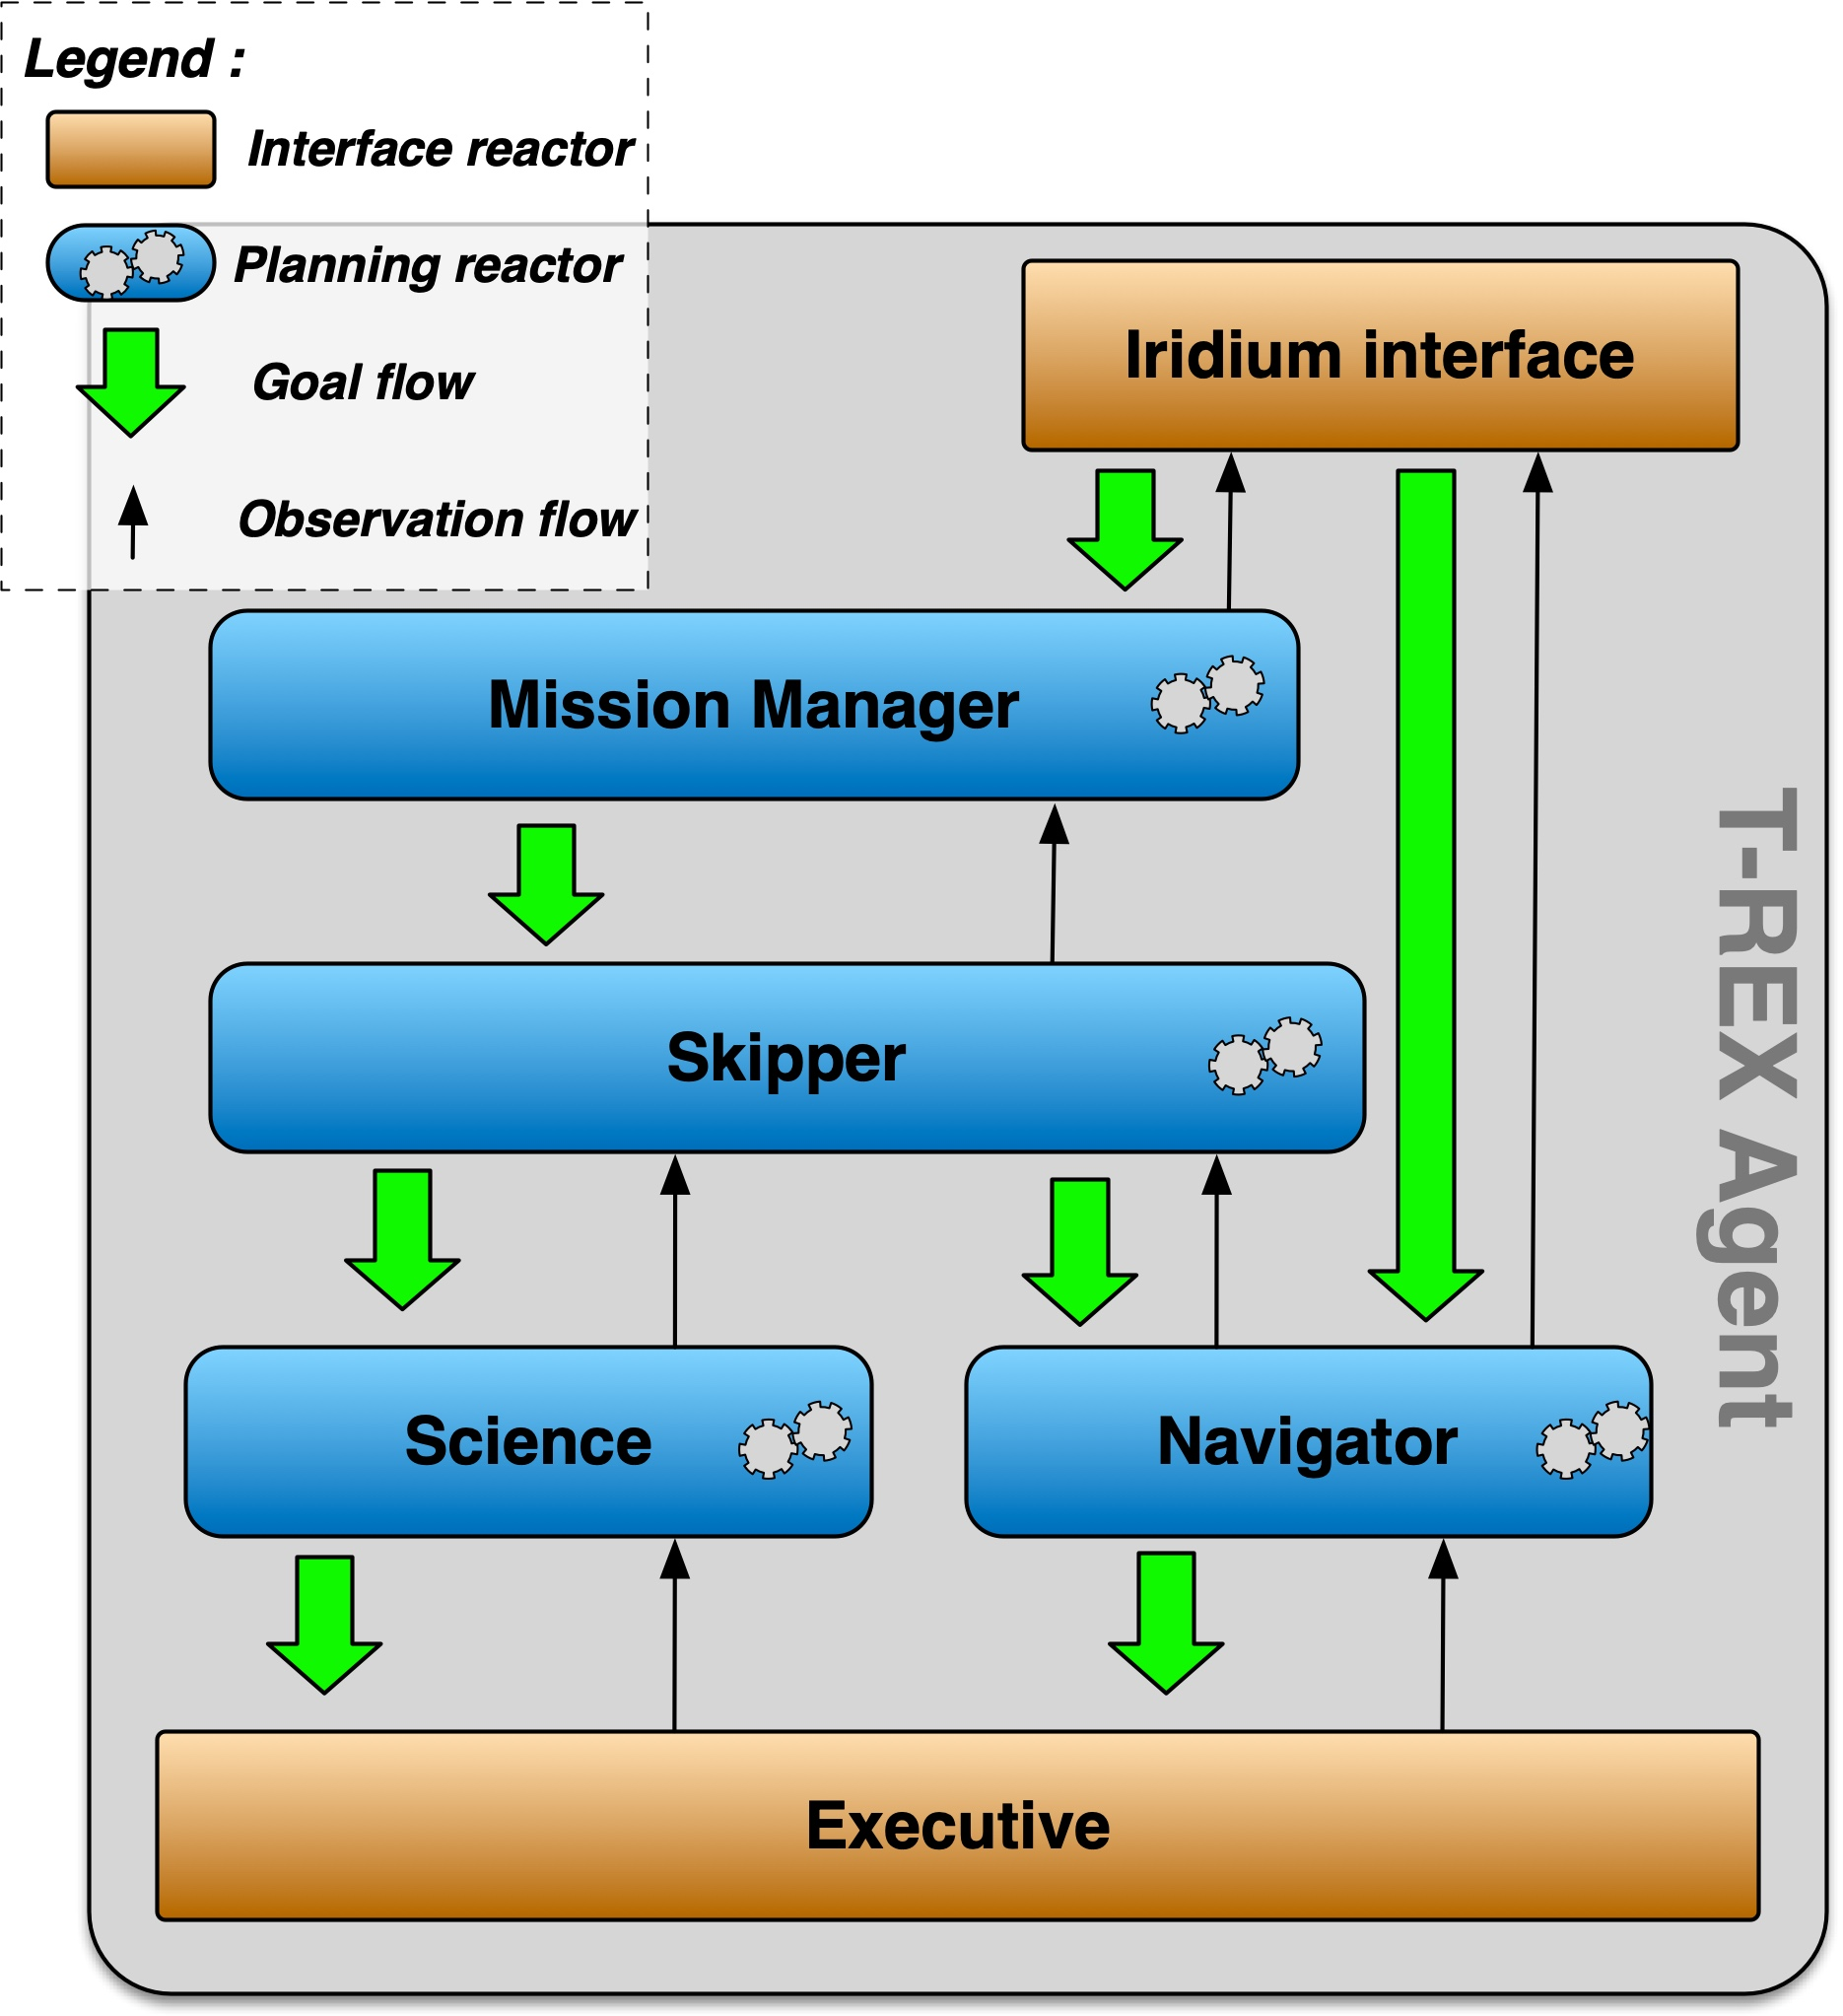
\includegraphics[scale=0.07]{fig/TREX-1.jpg}}
  \subfigure[]{\label{fig:components}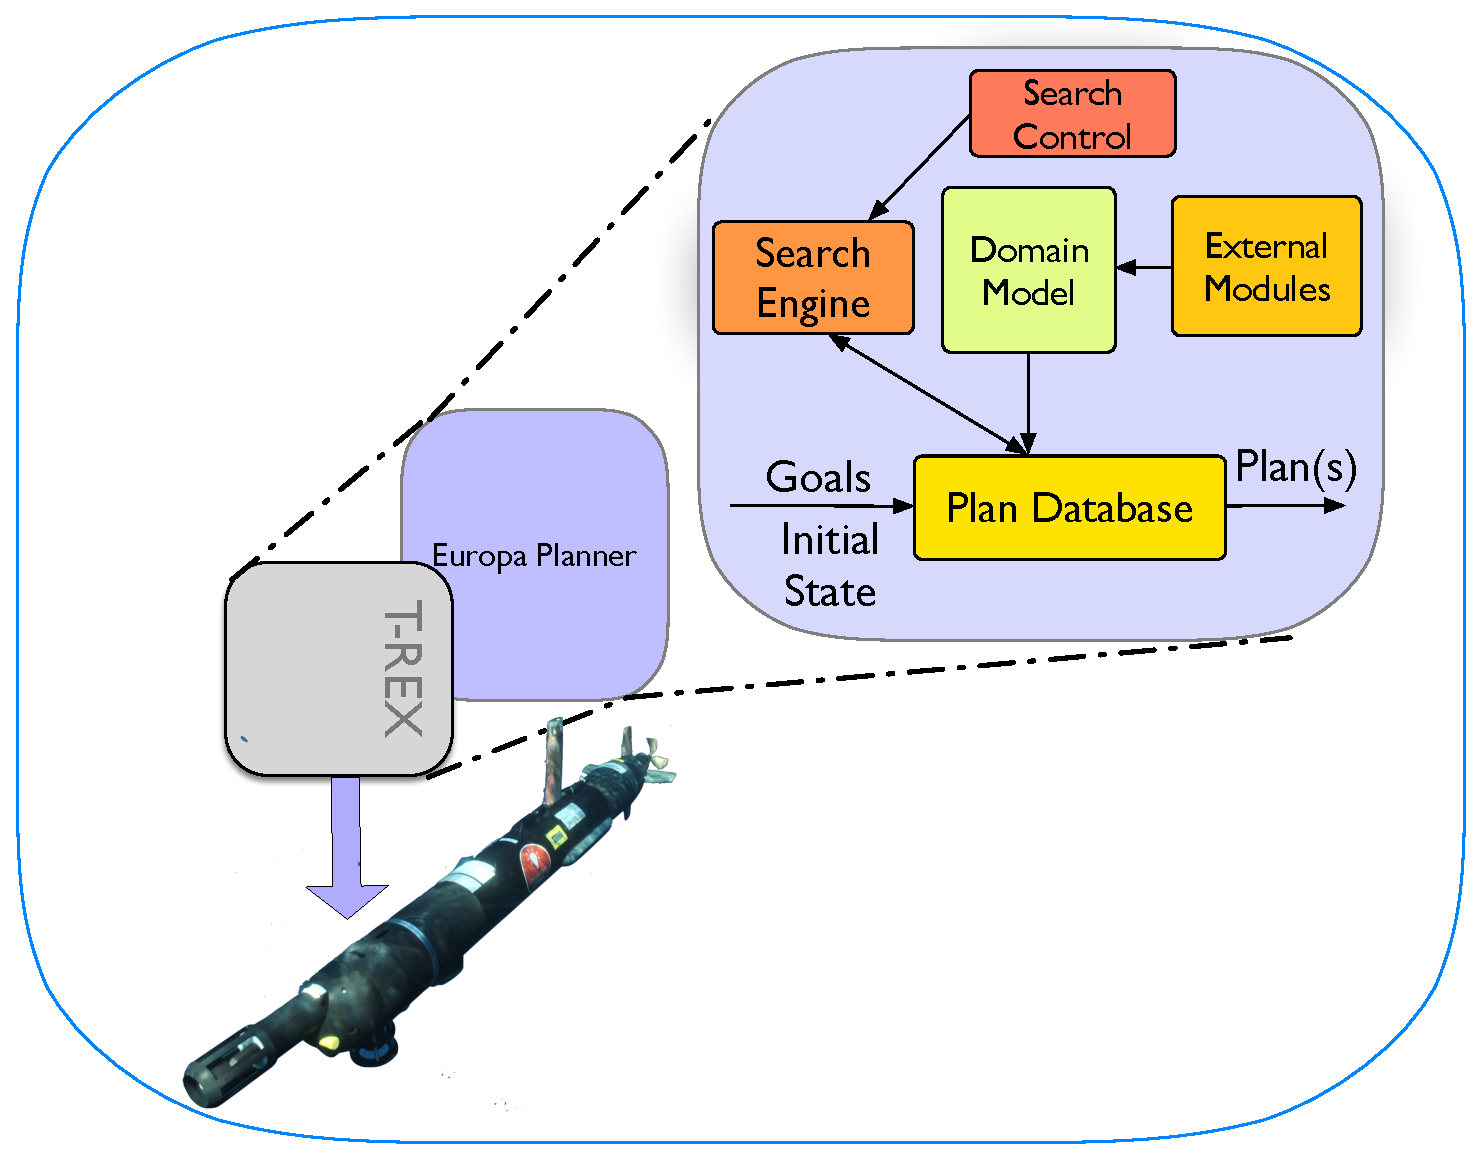
\includegraphics[scale=0.3]{fig/TREX-auv.pdf}}
  \caption{\subref{fig:vehicles} shows autonomous aerial and
    underwater vehicles from the Univ. of Porto, on a cruise in the
    Pacific in 2018.  % \subref{fig:agent} shows an example of a \rx
    % agent composed of multiple planning \emph{reactors} for
    % partitioned plan synthesis and execution. Each reactor has a
    % specific functional and temporal scope.
    \subref{fig:components} shows the hierarchy of architectural
    components for \rx \cite{py10,rajan12,rajan12b} which consists of
    an embedded planner on an AUV. Within each \rx component, resides
    a plan database and search engine, which comprise of
    representational primitives for constraint-based-planning.}
  \label{fig:ai-figs}
\end{figure}

In \proj we will use a range of well-tested networked autonomous
platforms (Fig. \ref{fig:vehicles}) operating with a substantial
operational legacy\footnote{\url{https://lsts.pt}} in coastal domains
\cite{pinto13,pinto14,sousa16,Ferreira2018,Pinto2018MultipleAV}. To
bind these unmanned assets, as well as users connecting from different
locations on shore, we rely on different components of the open source
\ls toolchain \cite{pinto2013lsts}. A brief summary of the toolchain
components is given in Table \ref{tab:toolchain}. In addition we will
leverage the considerable efforts in decision-making using Artificial
Intelligence (AI) methods targeting marine robotics. Our own efforts
revolve around operationalizing autonomous aerial, surface and
underwater platforms with embedded or off-shore decision-making
capacity which focus on the sense-plan-act control loop embedded on
autonomous vehicles.

\begin{table}[!t]
  \centering
  \footnotesize{
  \begin{tabular}{|p{1.8cm}|p{12.8cm}|p{0.75cm}|}\hline 
    \rowcolor{Gray}
    \bfseries Component & \bfseries Description & \bfseries Ref\\
    \hline
    \du&Low-level onboard navigation and control software embedded on
         all mobile platforms.&\cite{pinto2013lsts}\\
    \hline
    \nep&Shore/ship command and control system used to 
          visualize multiple autonomous heterogeneous vehicles. It can
          integrate data from external assets and other sources of
          information such AIS receivers, meteorological forecasting
          services and satellite imagery.&\cite{dias2005neptus}\\
    \hline
    \texttt{IMC}& Message-oriented, transport-agnostic binary protocol used 
    by all toolchain components both for inter-module and intra-module communications.
    &\cite{imc2009}\\
    \hline
    \rip& Cloud infrastructure used to aggregate and disseminate data from ongoing
          field deployments, as well as providing simplified web
          interfaces for following and controlling the operations using a
          browser; a stripped down alternative to \nep.&\cite{Pinto2018MultipleAV}\\
    \hline
  \end{tabular}
  \caption{\ls toolchain components critical for networked marine
    robotics and their description with citations to past work.}
  \label{tab:toolchain}
  }
\end{table}



We will use \rx (Teleo-Reactive EXecutive) an AI-based automated
planning/execution temporal framework to execute tasks
continuously. \rx is the only operational, \emph{deliberative} AI
based symbolic system in marine robotics anywhere, with a significant
record of operational use in the US, Portugal, and Norway. It is a
general purpose software system (Fig. \ref{fig:components}) that has
been demonstrated on terrestrial robots \cite{Meeussen10}, as well as
in space and underwater applications. It enables goal-oriented
commanding, balancing responsiveness to dynamic and unpredictable
environmental conditions with longer term mission goals. It does so by
synthesizing control actions onboard a robot and decomposing
high-level objectives sent from shore (or ship or even other
robots). It builds a task plan to actuate a robot while simultaneously
observing the evolving state of the robot's surroundings and
dynamically incorporating plan repair
\cite{py10,rajan12,rajan12b}. The symbolic planner at the heart of \rx
has a rich legacy from \nas having flown onboard the Deep Space 1
mission \cite{rajan00,jonsson00}, in addition to commanding the two
Mars Exploration Rovers (MER), \emph{Spirit} and \emph{Opportunity}
\cite{aichang04,bresina05}.

At its core, \rx has been used for dynamic feature tracking and
adaptive sampling to map fronts \cite{fronts11,smith14}, blooms
\cite{Das-2010-637}, ecological transport \cite{jdas12,jdas13} and
lagrangian drifters \cite{das10,das11a} while targeting multi-vehicle
deployments \cite{das11,Ferreira2018,pinto20}. Equally, the approaches
embedded in \rx use \emph{information theoretic} methods using marine
robots driven by a range of information sources
\cite{Das-2010-637,fronts11,olaya12,jdas12,jdas13,das15,fossum18,fossum19,fossum19b,fossum21}.
For \proj, we will use our reference work on adaptively sampling
dynamic underwater features, such as a sub-surface Chlorophyl max
(SCM) using Gaussian Process models \cite{fossum19} and Excursion Sets
\cite{fossum21}. \rx will be embedded on AUV's to detect and
dynamically track chlorophyll patches in the water-column, providing
high-resolution sampling data to be fed into the bio-geochemical
model. Predictions of where the patches might advect will then be
driven by ocean physics in the model and ground-truthed by the vehicle
in a subsequent iteration of the strategy to \texttt{tag},
\texttt{track} and \texttt{observe} strategy.



